% questions.tex —— 2006 年·普通高等学校招生考试·湖北卷理科 · 题目内容片段（无答案）
% 由 tools/generate_projects.py 依来源总账自 2006/2006_数学真题_湖北理_试题.md 生成，勿手改（改源 MD 后重跑）


\begin{gktip}
\textbf{来源及状态}：据固定 PDF 第 1–2 页逐题目视转录。固定文件 SHA-256 为 \texttt{670cd03dc447662d02befbf06b3e5ee8573cede1d4da521a9c03a104569e18e9}，与任务所给 Source ID 绑定；首页可见题签为“2006 普通高等学校招生考试（湖北卷理）”。题签与字节指纹仅标识本次读取的固定副本及其页内文字，不能认证发布者、版次、来源链或官方身份。此 PDF 所见为题面，不据此补答案、解析或分值。

\textbf{源页定位}：PDF 第 1 页（印刷页码 294）含 Q1–Q17；第 2 页（印刷页码 295）含 Q18–Q21。选择题 Q1–Q10，填空题 Q11–Q16，解答题 Q17–Q21。源页未见逐题分值或总分。

\textbf{图表}：Q15 的莱布尼茨三角形分数示例及 Q18 正方体示意图已按固定候选 PDF 重绘为 TikZ 矢量图；Q19 部分标准正态分布表按源页可见数值转录。Q18 源图未标点 P，图稿不补入该点。所有题图仍需随正式项目版面复核。
\end{gktip}

\gkpart{一、选择题}

\begin{question}
\gkti{1}已知向量 $\vec a=(\sqrt3,1)$，$\vec b$ 是不平行于 $x$ 轴的单位向量，且 $\vec a\cdot\vec b=\sqrt3$，则 $\vec b=$\mbox{（　　）}

（A）$\left(\dfrac{\sqrt3}{2},\dfrac12\right)$　（B）$\left(\dfrac12,\dfrac{\sqrt3}{2}\right)$　（C）$\left(\dfrac14,\dfrac{3\sqrt3}{4}\right)$　（D）$(1,0)$

\end{question}
\begin{question}
\gkti{2}若互不相等的实数 $a,b,c$ 成等差数列，$c,a,b$ 成等比数列，且 $a+3b+c=10$，则 $a=$\mbox{（　　）}

（A）$4$　（B）$2$　（C）$-2$　（D）$-4$

\end{question}
\begin{question}
\gkti{3}$\triangle ABC$ 的内角 $A$ 满足 $\sin 2A=\dfrac23$，则 $\sin A+\cos A=$\mbox{（　　）}

（A）$\dfrac{\sqrt{15}}3$　（B）$-\dfrac{\sqrt{15}}3$　（C）$\dfrac53$　（D）$-\dfrac53$

\end{question}
\begin{question}
\gkti{4}设 $f(x)=\lg\dfrac{2+x}{2-x}$，则 $f\left(\dfrac{x}{2}\right)+f\left(\dfrac{2}{x}\right)$ 的定义域为\mbox{（　　）}

（A）$(-4,0)\cup(0,4)$　（B）$(-4,-1)\cup(1,4)$

（C）$(-2,-1)\cup(1,2)$　（D）$(-4,-2)\cup(2,4)$

\end{question}
\begin{question}
\gkti{5}在 $\left(\sqrt{x}-\dfrac{1}{\sqrt[3]{x}}\right)^{24}$ 的展开式中，$x$ 的幂的指数是整数的项共有\mbox{（　　）}

（A）$3$ 项　（B）$4$ 项　（C）$5$ 项　（D）$9$ 项

\end{question}
\begin{question}
\gkti{6}关于直线 $m,n$ 与平面 $\alpha,\beta$，有以下四个命题：

① 若 $m\parallel\alpha$，$n\parallel\beta$ 且 $\alpha\parallel\beta$，则 $m\parallel n$；

② 若 $m\perp\alpha$，$n\perp\beta$ 且 $\alpha\perp\beta$，则 $m\perp n$；

③ 若 $m\perp\alpha$，$n\parallel\beta$ 且 $\alpha\parallel\beta$，则 $m\perp n$；

④ 若 $m\parallel\alpha$，$n\perp\beta$ 且 $\alpha\perp\beta$，则 $m\parallel n$。

其中真命题的序号是\mbox{（　　）}

（A）①②　（B）③④　（C）①④　（D）②③

\end{question}
\begin{question}
\gkti{7}设过点 $P(x,y)$ 的直线分别与 $x$ 轴的正半轴和 $y$ 轴的正半轴交于 $A,B$ 两点，点 $Q$ 与点 $P$ 关于 $y$ 轴对称，$O$ 为坐标原点，若 $\overrightarrow{BP}=2\overrightarrow{PA}$ 且 $\overrightarrow{OQ}\cdot\overrightarrow{AB}=1$，则点 $P$ 的轨迹方程是\mbox{（　　）}

（A）$3x^2+\dfrac32y^2=1\ (x>0,y>0)$　（B）$3x^2-\dfrac32y^2=1\ (x>0,y>0)$

（C）$\dfrac32x^2-3y^2=1\ (x>0,y>0)$　（D）$\dfrac32x^2+3y^2=1\ (x>0,y>0)$

\end{question}
\begin{question}
\gkti{8}有限集合 $S$ 中元素的个数记作 $\operatorname{card}(S)$，设 $A,B$ 都为有限集合，给出下列命题：

① $A\cap B=\varnothing$ 的充要条件是 $\operatorname{card}(A\cup B)=\operatorname{card}(A)+\operatorname{card}(B)$；

② $A\subseteq B$ 的必要条件是 $\operatorname{card}(A)\leqslant\operatorname{card}(B)$；

③ $A\nsubseteq B$ 的充分条件是 $\operatorname{card}(A)\leqslant\operatorname{card}(B)$；

④ $A=B$ 的充要条件是 $\operatorname{card}(A)=\operatorname{card}(B)$。

其中真命题的序号是\mbox{（　　）}

（A）①③④　（B）①②　（C）①④　（D）②③

\end{question}
\begin{question}
\gkti{9}已知平面区域 $D$ 由以 $A(1,3),B(5,2),C(3,1)$ 为顶点的三角形内部和边界组成。若在区域 $D$ 上有无穷多个点 $(x,y)$ 可使目标函数 $z=x+my$ 取得最小值，则 $m=$\mbox{（　　）}

（A）$-2$　（B）$-1$　（C）$1$　（D）$4$

\end{question}
\begin{question}
\gkti{10}关于 $x$ 的方程 $(x^2-1)^2-|x^2-1|+k=0$，给出下列四个命题：

① 存在实数 $k$，使得方程恰有 $2$ 个不同的实根；

② 存在实数 $k$，使得方程恰有 $4$ 个不同的实根；

③ 存在实数 $k$，使得方程恰有 $5$ 个不同的实根；

④ 存在实数 $k$，使得方程恰有 $8$ 个不同的实根。

其中假命题的个数是\mbox{（　　）}

（A）$0$　（B）$1$　（C）$2$　（D）$3$

\end{question}
\gkpart{二、填空题}

\begin{question}
\gkti{11}设 $x,y$ 为实数，且
\nopagebreak[4]
\[
\frac{x}{1-i}+\frac{y}{1-2i}=\frac{5}{1-3i},
\]
则 $x+y=$ \gkblank{}。

\end{question}
\begin{question}
\gkti{12}接种某疫苗后，出现发热反应的概率为 $0.80$，现有 $5$ 人接种该疫苗，至少有 $3$ 人出现发热反应的概率为 \gkblank{}。（精确到 $0.01$）

\end{question}
\begin{question}
\gkti{13}已知直线 $5x+12y+a=0$ 与圆 $x^2-2x+y^2=0$ 相切，则 $a$ 的值为 \gkblank{}。

\end{question}
\begin{question}
\gkti{14}某工程队有 $6$ 项工程需要先后单独完成，其中工程乙必须在工程甲完成后才能进行，工程丙必须在工程乙完成后才能进行，又工程丁必须在工程丙完成后立即进行。那么安排这 $6$ 项工程的不同排法种数是 \gkblank{}。（用数字作答）

\Needspace{0.4\textheight}
\end{question}
\begin{question}
\gkti{15}将杨辉三角中的每一个数 $C_n^r$ 都换成分数 $\dfrac{1}{(n+1)C_n^r}$，就得到一个如下图所示的分数三角形，成为莱布尼茨三角形。从莱布尼茨三角形可看出
\nopagebreak[4]
\[
\frac{1}{(n+1)C_n^r}+\frac{1}{(n+1)C_n^{r+1}}=\frac{1}{nC_{n-1}^r},
\]
\Needspace{5\baselineskip}
其中 $x=\dfrac{1}{nC_{n-1}^r}$。令
\nopagebreak[4]
\[
a_n=\frac13+\frac1{12}+\cdots+\frac{1}{nC_{n-1}^{2}}+\frac{1}{(n+1)C_n^{2}},
\]
则 $\displaystyle\lim_{n\to\infty}a_n=$ \gkblank{}。
\nopagebreak[4]
\begin{center}% 2006 湖北理科第15题：源图中的莱布尼茨三角形分数排列。
\begin{tikzpicture}[x=0.86cm, y=0.78cm, font=\small]
  \node at (0, 0) {$\dfrac{1}{1}$};

  \node at (-0.5, -1) {$\dfrac{1}{2}$};
  \node at ( 0.5, -1) {$\dfrac{1}{2}$};

  \node at (-1, -2) {$\dfrac{1}{3}$};
  \node at ( 0, -2) {$\dfrac{1}{6}$};
  \node at ( 1, -2) {$\dfrac{1}{3}$};

  \node at (-1.5, -3) {$\dfrac{1}{4}$};
  \node at (-0.5, -3) {$\dfrac{1}{12}$};
  \node at ( 0.5, -3) {$\dfrac{1}{12}$};
  \node at ( 1.5, -3) {$\dfrac{1}{4}$};

  \node at (-2, -4) {$\dfrac{1}{5}$};
  \node at (-1, -4) {$\dfrac{1}{20}$};
  \node at ( 0, -4) {$\dfrac{1}{30}$};
  \node at ( 1, -4) {$\dfrac{1}{20}$};
  \node at ( 2, -4) {$\dfrac{1}{5}$};

  \node at (-2.5, -5) {$\dfrac{1}{6}$};
  \node at (-1.5, -5) {$\dfrac{1}{30}$};
  \node at (-0.5, -5) {$\dfrac{1}{60}$};
  \node at ( 0.5, -5) {$\dfrac{1}{60}$};
  \node at ( 1.5, -5) {$\dfrac{1}{30}$};
  \node at ( 2.5, -5) {$\dfrac{1}{6}$};

  \node at (-3, -6) {$\dfrac{1}{7}$};
  \node at (-2, -6) {$\dfrac{1}{42}$};
  \node at (-1, -6) {$\dfrac{1}{105}$};
  \node at ( 0, -6) {$\dfrac{1}{140}$};
  \node at ( 1, -6) {$\dfrac{1}{105}$};
  \node at ( 2, -6) {$\dfrac{1}{42}$};
  \node at ( 3, -6) {$\dfrac{1}{7}$};

  \node at (0, -7) {$\cdots\cdots$};
\end{tikzpicture}
\end{center}
\nopagebreak[4]
\end{question}
\begin{question}
\gkti{16}设函数
\nopagebreak[4]
\[
f(x)=\vec a\cdot(\vec b+\vec c),\quad
\vec a=(\sin x,-\cos x),\quad
\vec b=(\sin x,-3\cos x),\quad
\vec c=(-\cos x,\sin x),\quad x\in\mathbb R.
\]

（1） 求函数 $f(x)$ 的最大值和最小正周期；

（2） 将函数 $f(x)$ 的图像按向量 $\vec d$ 平移，使平移后得到的图像关于坐标原点成中心对称，求长度最小的 $\vec d$。

\end{question}
\gkpart{三、解答题}

\begin{question}
\gkti{17}已知二次函数 $y=f(x)$ 的图象经过坐标原点，其导函数为 $f'(x)=6x-2$，数列 $\{a_n\}$ 的前 $n$ 项和为 $S_n$，点 $(n,S_n)\ (n\in\mathbb N^*)$ 均在函数 $y=f(x)$ 的图象上。

（1） 求数列 $\{a_n\}$ 的通项公式；

（2） 设 $b_n=\dfrac{m}{a_na_{n+1}}$，$T_n$ 是数列 $\{b_n\}$ 的前 $n$ 项和，求使得 $T_n<\dfrac{m}{20}$ 对所有 $n\in\mathbb N^*$ 都成立的最小正整数 $m$。

\Needspace{0.4\textheight}
\end{question}
\begin{question}
\gkti{18}如图，在棱长为 $1$ 的正方体 $ABCD-A_1B_1C_1D_1$ 中，$P$ 是侧棱 $CC_1$ 上的一点，$CP=m$。

（1） 试确定 $m$，使直线 $AP$ 与平面 $BDD_1B_1$ 所成角的正切值为 $3\sqrt2$；

（2） 在线段 $A_1C_1$ 上是否存在一个定点 $Q$，使得对任意的 $m$，$D_1Q$ 在平面 $APD_1$ 上的射影垂直于 $AP$，并证明你的结论。
\nopagebreak[4]
\begin{center}% 2006 湖北理科第18题：源图所示正方体及上底面对角线；点 P 未画在源图中。
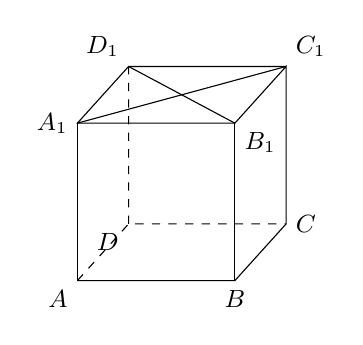
\begin{tikzpicture}[x=1cm, y=1cm, font=\small]
  \coordinate (A)  at (0,0);
  \coordinate (B)  at (2,0);
  \coordinate (C)  at (2.65,0.72);
  \coordinate (D)  at (0.65,0.72);
  \coordinate (A1) at (0,2);
  \coordinate (B1) at (2,2);
  \coordinate (C1) at (2.65,2.72);
  \coordinate (D1) at (0.65,2.72);

  % 可见棱
  \draw (A) -- (B) -- (C) -- (C1) -- (B1) -- (A1) -- (D1) -- (C1);
  \draw (A) -- (A1);
  \draw (B) -- (B1);
  % 源图中的隐藏棱
  \draw[dashed] (A) -- (D) -- (C) (D) -- (D1);
  % 顶面两条对角线
  \draw (A1) -- (C1);
  \draw (D1) -- (B1);

  \node[below left] at (A) {$A$};
  \node[below] at (B) {$B$};
  \node[right] at (C) {$C$};
  \node[below left] at (D) {$D$};
  \node[left] at (A1) {$A_1$};
  \node[below right] at (B1) {$B_1$};
  \node[above right] at (C1) {$C_1$};
  \node[above left] at (D1) {$D_1$};
\end{tikzpicture}
\end{center}
\nopagebreak[4]
\end{question}
\begin{question}
\gkti{19}在某校举行的数学竞赛中，全体参赛学生的竞赛成绩近似服从正态分布 $N(70,100)$。已知成绩在 $90$ 分以上（含 $90$ 分）的学生有 $12$ 名。

（1） 试问此次参赛学生总数约为多少人？

（2） 若该校计划奖励竞赛成绩排在前 $50$ 名的学生，试问设奖的分数线约为多少分？

可供查阅的（部分）标准正态分布表 $\Phi(x_0)=P(x<x_0)$：

\begin{center}
\begin{tabular}{lrrrrr}
\toprule
$x_0$ & 0 & 1 & 2 & 3 & 4 \\
\midrule
1.2 & 0.8849 & 0.8869 & 0.888 & 0.8907 & 0.8925 \\
1.3 & 0.9032 & 0.9049 & 0.9066 & 0.9082 & 0.9099 \\
1.4 & 0.9192 & 0.9207 & 0.9222 & 0.9236 & 0.9251 \\
1.9 & 0.9713 & 0.9719 & 0.9726 & 0.9732 & 0.9738 \\
2.0 & 0.9772 & 0.9778 & 0.9783 & 0.9788 & 0.9793 \\
2.1 & 0.9821 & 0.9826 & 0.9830 & 0.9834 & 0.9838 \\
\bottomrule
\end{tabular}
\end{center}

\begin{center}
\begin{tabular}{lrrrrr}
\toprule
$x_0$ & 5 & 6 & 7 & 8 & 9 \\
\midrule
1.2 & 0.8944 & 0.8962 & 0.8980 & 0.8997 & 0.9015 \\
1.3 & 0.9115 & 0.9131 & 0.9147 & 0.9162 & 0.9177 \\
1.4 & 0.9265 & 0.9278 & 0.9292 & 0.9306 & 0.9319 \\
1.9 & 0.9744 & 0.9750 & 0.9756 & 0.9762 & 0.9767 \\
2.0 & 0.9798 & 0.9803 & 0.9808 & 0.9812 & 0.9817 \\
2.1 & 0.9842 & 0.9846 & 0.9850 & 0.9854 & 0.9857 \\
\bottomrule
\end{tabular}
\end{center}

\end{question}
\begin{question}
\gkti{20}设 $A,B$ 分别为椭圆 $\dfrac{x^2}{a^2}+\dfrac{y^2}{b^2}=1\ (a,b>0)$ 的左、右顶点，椭圆长半轴的长等于焦距，且 $x=4$ 为它的右准线。

（1） 求椭圆的方程；

（2） 设 $P$ 为右准线上不同于点 $(4,0)$ 的任意一点，若直线 $AP,BP$ 分别与椭圆相交于异于 $A,B$ 的点 $M,N$，证明点 $B$ 在以 $MN$ 为直径的圆内。

\end{question}
\begin{question}
\gkti{21}设 $x=3$ 是函数 $f(x)=(x^2+ax+b)e^{3-x}\ (x\in\mathbb R)$ 的一个极值点。

（1） 求 $a$ 与 $b$ 的关系式（用 $a$ 表示 $b$），并求 $f(x)$ 的单调区间；

（2） 设 $a>0$，$g(x)=\left(a^2+\dfrac{25}{4}\right)e^x$。若存在 $\xi_1,\xi_2\in[0,4]$ 使得 $|f(\xi_1)-g(\xi_2)|<1$ 成立，求 $a$ 的取值范围。

\end{question}